\documentclass{beamer}
\usetheme{metropolis}

\usepackage{tikz}

\usepackage{tikz}
\usepackage{animate}
\usepackage{ifthen}

\usepackage[T1]{fontenc}
\usepackage[utf8]{inputenc}

\usepackage{graphicx}
\graphicspath{ {./} }

\usepackage{listings}

\def\bitcoinA{%
  \leavevmode
  \vtop{\offinterlineskip %\bfseries
    \setbox0=\hbox{B}%
    \setbox2=\hbox to\wd0{\hfil\hskip-.03em
    \vrule height .3ex width .15ex\hskip .08em
    \vrule height .3ex width .15ex\hfil}
    \vbox{\copy2\box0}\box2}}

\lstset{basicstyle=\ttfamily}

\makeatletter
\def\verbatim@font{\footnotesize\ttfamily}
\makeatother

\title{Laserowy kotek}
\subtitle{czyli jak zrobić grę w wielbłądzie}
\author{Weronika Jakimowicz}
\date{Luty 2024}


\begin{document}

\begin{frame}
  \maketitle 
  \begin{tikzpicture}[overlay, remember picture]
    \node at (9,8) {
\includegraphics[width=0.3\textwidth]{tytul_obrazek.jpg}};
    \node at (9, 3.5) {\reflectbox{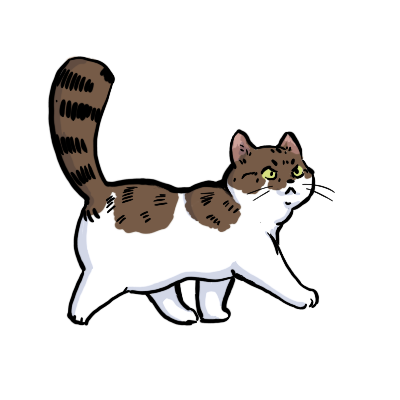
\includegraphics[width=0.4\textwidth]{moj_kotek.png}}};
  \end{tikzpicture}
\end{frame}

\begin{frame}{Co się udało zrobić?}
  \begin{enumerate}
    \item Kycia wznosi się 

      i upada
    \item Czarne Psy pojawiają

      się i znikają
    \item Kycia może inwestować w {\bitcoinA}itcoin
    \item Laser
    \item Licznik punktów i przebieg Kyci
    \item Można przegrać (tylko)
  \end{enumerate}
  \begin{tikzpicture}[overlay, remember picture]
    \node at (10, 0) {
\includegraphics[width=0.4\textwidth]{piesio_01.png}};
    \node at (8.1, 5.1) { \rotatebox{-15}{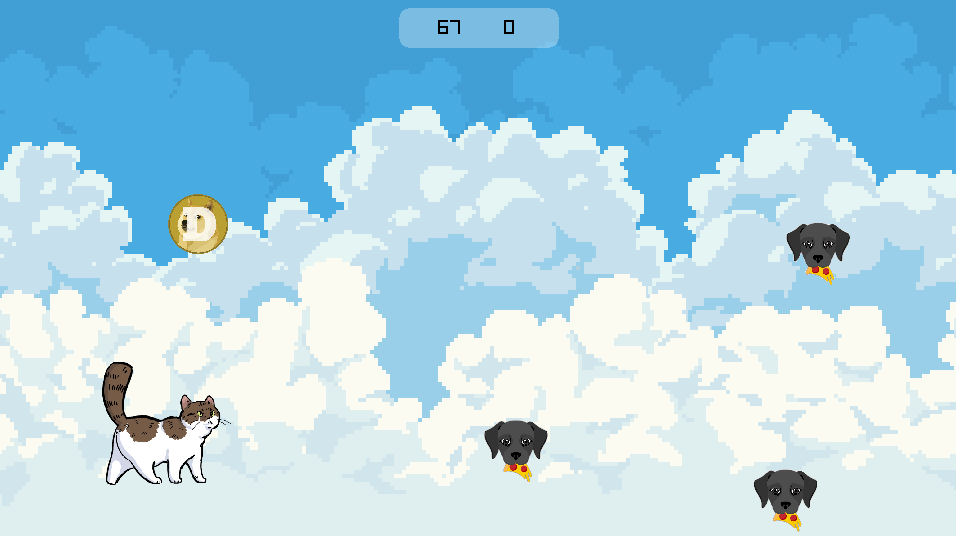
\includegraphics[width=0.65\textwidth]{pokazowka.png}} };
  \end{tikzpicture}
\end{frame}

\begin{frame}{Prezentacja gotowego projektu}
  \begin{center}
    \emph{To jest ten moment kiedy pokazuję grę}
  \end{center}
\end{frame}

\begin{frame}{Struktura}
  \begin{center}
    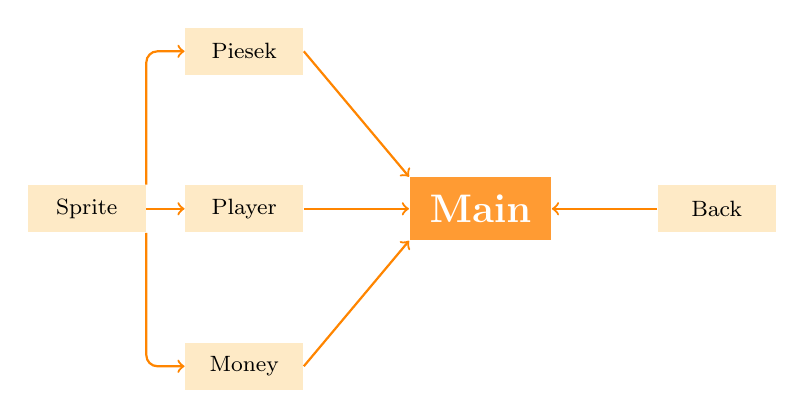
\begin{tikzpicture}[
        sqn/.style={rectangle, fill=yellow!25!orange!20, minimum width=15mm, minimum height=6mm},
        sqn2/.style={rectangle, fill=orange!60!red!70!yellow!80, minimum width=18mm, minimum height=8mm},
        ]

      \node[sqn] (sp) at (0, -2) {\footnotesize Sprite};
      \node[sqn] (pi) at (2, 0) {\footnotesize Piesek};
      \node[sqn] (pl) at (2, -2) {\footnotesize Player};
      \node[sqn] (mo) at (2, -4) {\footnotesize Money};

      \draw[rounded corners, ->, thick, orange!40!red!60!yellow] (sp.north east) |- (pi.west);
      \draw[rounded corners, ->, thick, orange!40!red!60!yellow] (sp.east) -- (pl.west);
      \draw[rounded corners, ->, thick, orange!40!red!60!yellow] (sp.south east) |- (mo.west);

      \node[sqn] (ba) at (8, -2) {\footnotesize Back};

      \node[sqn2] (main) at (5, -2) {\textbf{\Large\color{white}Main}};

      \draw[->, thick, orange!40!red!60!yellow] (ba.west) -- (main.east);

      \draw[->, thick, orange!40!red!60!yellow, rounded corners] (pi.east) -- (main.north west);
      \draw[->, thick, orange!40!red!60!yellow] (pl.east) -- (main.west);
      \draw[->, thick, orange!40!red!60!yellow, rounded corners] (mo.east) -- (main.south west);
    \end{tikzpicture}
    \begin{tikzpicture}[overlay, remember picture] 
      \node[opacity=0.7] at (-0.5, 5) {\reflectbox{
\includegraphics[width=0.4\textwidth]{kycia_01.png}}};
    \end{tikzpicture}
  \end{center}
\end{frame}

\begin{frame}{Problemy}
  \begin{itemize}
    \item Pauzowanie a rozwiązanie problemu ze zmiennymi \lstinline{player} etc.
    \item 
\includegraphics[height=3mm]{dune_logo.png} wrzuca wszystkie pliki do \lstinline{_build/default/src/...}
    \item Używanie 
\includegraphics[height=3mm]{dune_logo.png} do kompilacji a pliki \lstinline{*.mli}
    \item Rekordy nie mają od razu pól prywatnych, publicznych etc.
  \end{itemize}

  \begin{tikzpicture}[overlay, remember picture]
    \node at (9, -0.5) {\rotatebox{-20}{
\includegraphics{worm.png}}};
    \node at (9.5, 5.3) { \rotatebox{-20}{
\includegraphics[width=0.28\textwidth]{sun.png}} };
    \node at (1.2, -0.7) { 
\includegraphics[width=0.3\textwidth]{desert.png} };
  \end{tikzpicture}
\end{frame}

\begin{frame}[fragile]{Przyjemności}
  \begin{itemize}
    \item \lstinline{List.fold_left} bardzo fajnie działa do iterowania przez listę wrogów
    \item \lstinline{raylib} jest przyjemniaśny
    \item Mój ulubieniec:
      \begin{lstlisting}[
      language=caml, 
      frame=leftline,
      rulecolor=\color{orange!40!black}, 
      breaklines=true,
      keywordstyle=\bfseries\color{orange!70!red},
      commentstyle=\color{gray},
      backgroundcolor=\color{lightgray!20},
      ]
type move_direction = 
  | Jump
  | Fall 
  | Stationary
      \end{lstlisting}
  \end{itemize}

  \begin{tikzpicture}[overlay, remember picture]
    \node at (8, 0.5) {\rotatebox{-5}{
\includegraphics[width=0.4\textwidth]{sassy_camel.png}}};
    \node at (6, 2) {\rotatebox{10}{
\includegraphics[width=0.1\textwidth]{green.png}}};
    \node at (7, 2.5) {\rotatebox{-20}{
\includegraphics[width=0.05\textwidth]{green.png}}};
  \end{tikzpicture}
\end{frame}

\end{document}
